 % - Components and their Interfaces
 %   - Parent subnet node
 %   - Child subnet node
 %   - IPC module
 %   - Subnet actor
 \section{Components and their Interfaces}
 \label{sec:components}

We now focus on the interaction between two subnets in a parent-child relation.
This interaction comprises running the subnets, observing each other's replicated state,
constructing \pofsFull, submitting the necessary transactions, and modifying the replicated state accordingly. To enable this interaction, \ipc consists of 
several components and interfaces between them, which we  
illustrate in \Cref{fig:interfaces}.\\

\begin{figure}[ht]
     \centering
     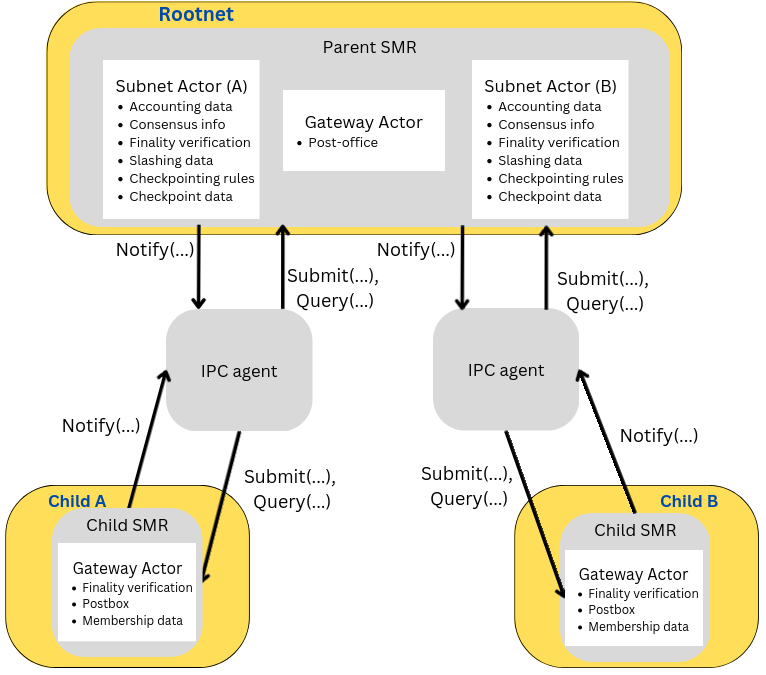
\includegraphics[width=0.75\textwidth]{compsintf-2subnets}
     \caption{The basic \ipc components and their interfaces in an example with one parent and 2 child subnets (A and B).}
     \label{fig:interfaces}
 \end{figure}

\subsection{Components}

\ipc components consist of three types  of \emph{processes} and two types of \emph{actors} (smart contracts).

\subsubsection{Processes}

\begin{enumerate}
    
    \item \textbf{Parent replica:} The process that executes the SMR protocol of the parent subnet. It has a copy of the parent's replicated state, participates in receiving and ordering transactions and updates the replicated state (including the \sa \dapp) accordingly.
    
    \item \textbf{Child replica:} The process that executes the SMR protocol of the child subnet. It has a copy of the child's replicated state, participates in receiving and ordering transactions and updates the replicated state (including the \gw \dapp) accordingly.

    \item \textbf{\ipc agent:} The process that mediates the interactions between the two subnets.
    It has access to the replicated states of both the parent and the child
    (e.g., by sharing a trust domain with a child and a parent replica, or by downloading the replicated state from other replicas)
    and acts as an SMR client (i.e., submits transactions) to both subnets.
    It is also responsible for constructing \pofsFull (which might involve communication with other processes).

\end{enumerate}
 
 \subsubsection{Actors (smart contracts)}

\begin{enumerate}
    \item \textbf{Subnet actor (\sa):} The smart contract in the parent subnet's replicated state
    that stores all information about the child subnet that the parent subnet needs.
    The \sa is created by the \gw (see below) and its functions are invoked by transactions the \ipc agent.
    The state of the \sa includes:
    \begin{itemize}

        \item \emph{Accounting data.}
        This data describes the value that has been deposited to the child.
        It is considered locked inside the SA until it is withdrawn from the child.
        This data might consist of just a single value representing the sum of all such coins (``aggregated accounts'' approach),
        but might also contain finer-grained information about balances for each account in the child subnet (``segregated accounts'' approach).
        %We continue with the non-custodial approach as the other can be viewed as a specific limitation of it.

        \del{\item \emph{Governance account.}
        This account facilitates the economic design of a subnet.
        It can be used for collecting fees or making payments to accounts of participants that perform operations on behalf of the child subnet.
        For example, when an IPC agent submits (and thus pays for) transaction linking a child's checkpoint to the parent's replicated state,
        the IPC actor logic might reimburse the associated account}

        \item \emph{Ordering protocol (subnet consensus) data.}
        This is the data (or a pointer to it) that is needed to run the ordering protocol of the child subnet.
        It is ordering protocol-specific, but is generally expected to contain information such as
        \begin{itemize}
            \item The ordering protocol used by the subnet.
            \item Subnet configuration such as the validator set, voting rights, and collateral deposits.
            \item Subnet governance mechanisms, e.g., transaction fees, block rewards, conditions for participation.
        \end{itemize}
        \TODO{Mention our reference implementation as a concrete example here, saying what information it stores.}

        \item \emph{Child state finality verification.} Logic to verify that a given child's replicated state/\tx is final.
        or that a particular \tx has been definitively included in the child's state.
        We expect that this logic will verify a \pof submitted (through transactions) by one or more IPC agents to the \sa.
        % For this, we will use the function \sa.\verifyGfinal{\tx}{\prf} which excepts as arguments a transaction (or state) and a \prf, and outputs True if \tx is considered globally final in the child subnet and False otherwise. This function must only depend on its inputs and the internal state of~\sa. For example, \prf is a threshold signature that can be verified against the set of validators in~\sa.
          
        \item \emph{Slashing.}
        \begin{itemize}
            \item List of slashable misbehaviors and a proving methodology. That is, for each slashable misbehavior there is a definition of what constitutes a valid proof of misbehavior (\pom).
            \item Penalties for misbehavior and rewards for reporting \pom, as well as the logic performing the  actions necessary for slashing in the parent subnet.
        \end{itemize}
        \item \emph{Checkpointing.}
        \begin{itemize}
            \item Child subnet's checkpoint data or a pointer to it.
            \item Checkpoint validity rules (and logic enforcing them).
            E.g., ``Checkpoints must be at least every~$\Delta$ subnet blocks apart'', or ``A checkpoint must contain a hash of the previous checkpoint''.
            % the checkpoint's $L_2$ distance from the previous is larger than~$L$.
            %\item Fee payments for checkpoints.
        \end{itemize}
    \end{itemize}
    \item \textbf{IPC coordinator/gateway actor (\gw):} a smart contract that exists in every subnet in the \ipc hierarchy and contains all information and logic the subnet itself needs to hold in order to be part of \ipc. The state of the \gw includes:
    \begin{itemize}
        \item
        \emph{Membership data} defining the set of replicas running the \gw's subnet.
        This may include the identities of the replicas, their network addresses, weights of their votes in the executed consensus protocol (e.g., storage power table, or stake power table), and other subnet-specific membership information.

        \item \emph{Parent state finality verification.} Analogously to the \sa's child state finality verification logic,
        this is the logic to verify that a state/\tx is final in the parent subnet,
        using a \pof submitted as transaction(s) to the child subnet by the IPC agent(s).
        % For this, we will use the function \gw.\verifyPfinal{\tx}{\prf} which excepts as arguments a transaction (or state) and a \prf, and outputs True if \tx is considered globally final in the parent subnet and False otherwise. This function must only depend on its inputs (and perhaps some internal state of~\gw).
        \item \emph{Inter-subnet transactions service} (denoted \postoffice).
        The \gw contains a registry of subnets and a functionality that can be used to transfer data from one subnet to another. 
        The \postoffice specifies the methods and the state locations that are used for these services.
        This functionality is required for the communication of two smart contracts across subnets.%
        % In particular, consider the following case involving a smart contract.%
\footnote{When inter-subnet data transfer happens between users, they can actively participate in the propagation by submitting transactions to the parent and child subnets. Smart contracts, on the other hand, do not have that power and, therefore, cannot communicate inter-subnets as efficiently as users (\eoa).}
    \end{itemize}
\end{enumerate}

% OLD VERSION:
% \begin{enumerate}
%     \item \textbf{\ipc agent:} The software that is in charge of the interactions between the two blockchains. This includes, for example, observers for the parent and child subnets. (Note that it is a process and not a smart contract). The \ipc agent is a piece of software that mediates the interactions between the child and parent \smr software modules.    
%     \item \textbf{Parent \smr replica:} The software that runs the parent blockchain. Note that this module also entails the interaction with the \ipc smart contract~\sa, which is maintained at the parent subnet. Any update that the parent process performs on \sa is notified to the \ipc agent.
%     \item \textbf{Child \smr replica:} The software that runs the child blockchain. Note that some of the rules the child blockchain must satisfy are listed in~\sa. Any output operation (withdraw, checkpoint) is notified to the parent process through the \ipc agent. 
% %    \item \textbf{IPC smart contract / subnet actor (\sa):} The smart contract implementation that is running on the parent blockchain. It is invoked only through transactions that are included in the parent blockchain.
%     \item \textbf{IPC subnet actor (\sa):} The smart contract implementation that is running on the parent blockchain. It is invoked only through transactions that are included in the parent blockchain.
%     \item \textbf{IPC coordinator/gateway actor (\gw):} a smart contract that exists in every non-leaf subnet in the \ipc hierarchy and contains methods facilitating inter-subnet operations.	
% \end{enumerate}

\subsection{Interfaces}

We now describe the interfaces of the Gateway Actor (\gw) and the Subnet Actor (\sa), by listing the methods that can be invoked through transactions submitted to their respective subnets,
as well as that of the IPC Agent process, by listing the events it reacts to.
The other two processes, the parent and child replica, interact with the IPC Agent by having the IPC Agent observe the relevant parts of parent's and child's replicated state.
The parent and child replicas do not perform any IPC-specific tasks themselves, except for providing the data necessary for IPC Agents to construct \pofsFull.

\paragraph{Notation.} We refer to an account $a$ in the replicated state of subnet $S$ as $S.a$.
To denote a Function a of Smart Contract in the replicated state of a Subnet, we write $Subnet.SmartContract.Function$.
E.g., the \gw's function $CreateChild$ in subnet $P$ is denoted $P.\gw.CreateChild$.
We also use this notation for a transaction $tx$ submitted to subnet $P$ that invokes the function, e.g., $tx = P.\gw.CreateChild(P/C, params)$.

\subsubsection{Gateway Actor (\gw)}

\begin{algorithm}[H]
\footnotesize
\caption{\gw interface}\label{alg:gw-interface}
  \DontPrintSemicolon
  \SetKwProg{Component}{$\blacktriangleright$ \bf}{:}{\KwRet}
  \SetKwFor{UponKW}{}{}{fintq}
  \SetKw{Trigger}{trigger}
  \Component{\gw}{
    \UponKW{CreateChild(name, params)}{
        Creates a new \sa with the given name and subnet-specific parameters (such as initial membership, etc.).
        The subnet governed by the created \sa will be considered the child of the subnet of this \gw.
    }
    \UponKW{RemoveChild(name)}{
        \matej{Is it meaningful to have this functionality at all?}%\arp{TLDR: killing a subnet is not necessarily trivial.\\ In our current implementation a client of a child subnet assumes $f<n/3$ where $n$ is the validators set at the child, but this is not necessarily a requirement of subnets. For example, state (lightning, payment) channels should be a specific case of subnets in which the set of validators = all clients of the subnet. In state channels, validators are required to sign in order to change the state (full safety but no liveness if $f\geq 1$) -- except for killing the subnet, allowing correct validators to withdraw with latest checkpoint without deadlocking their state in the corrupted subnet. This can be done with timelocks in an orderly manner. AFAIK Plasma chains even have the same functionality for clients to be able to circumvent a corrupted child subnet they belong to and skip to parent. }
    }
    \UponKW{Joined(identity, metadata, \pof)}{
        For subnets with explicit membership defined by the \sa in their parent, if \emph{\pof} is valid,
        updates the membership data of the \gw to include the replica with \emph{identity} and the associated \emph{metadata}.
        A valid \pof means that \emph{\sa.Join(identity, ..., ...)} has been successfully invoked in the parent's replicated state.
    }
    \UponKW{Leave(identity)}{
        For subnets with explicit membership defined by the \sa in their parent, removes the replica with \emph{identity} from this subnet's membership.
    }
    \UponKW{Deposited(amt, dest, \pof)}{
        If \emph{\pof} is valid, adds \emph{amt} newly minted coins to account \dest.
        A valid \pof means that a corresponding \emph{SA.Deposit(..., amt, dest)} has been successfully invoked in the parent's replicated state.
    }
    \UponKW{Withdraw(src, amt, dest)}{
        Burns \emph{amt} coins from account \emph{src} to be returned to the \dest account in the parent subnet.
    }
    \UponKW{Propagate(tx)}{
        Adds the cross-net transaction \emph{tx} to the list of transactions to be submitted to the another subnet.
        (The IPC agents observing the state of this subnet will pick it up from here and do the actual submission.)
    }
}
\end{algorithm}

\subsubsection{Subnet Actor (\sa)}

\begin{algorithm}[H]
\footnotesize
\caption{\sa interface (governing subnet $C$)}\label{alg:sa-interface}
  \DontPrintSemicolon
  \SetKwProg{Component}{$\blacktriangleright$ \bf}{:}{\KwRet}
  \SetKwFor{UponKW}{}{}{fintq}
  \SetKw{Trigger}{trigger}
  \Component{\sa}{
    \UponKW{Join(identity, src, collateral)}{
        For subnets with explicit membership defined by the \sa, adds the replica with the given \emph{identity} to the replica set of the subnet governed by this \sa.
        Join also locks \emph{collateral} coins in the \emph{src} account the will only be released when the replica leaves.
    }
    \UponKW{Left(identity, \pof)}{
        For subnets with explicit membership defined by the \sa, if \emph{\pof} is valid, adds the replica with the given \emph{identity} to the replica set of the subnet governed by this \sa.
        The \pof proves that the corresponding \emph{C.\gw.Leave(identity)} has been successfully invoked and the replica with the given \emph{identity} is not running subnet $C$ any more.
    }
    \UponKW{Deposit(src, amt, dest)}{
        Locks \emph{amt} coins on account \src to be deposited to the \dest account on the child subnet.
    }
    \UponKW{Withdrawn(amt, dest, \pof)}{
        If \emph{\pof} is valid (meaning that a corresponding \emph{C.\gw.Withdraw(..., amt, dest)} has been successfully invoked),
        unlocks \emph{amt} coins on the \dest account.
    }
    \UponKW{Checkpoint(chkp, \pof)}{
        If \emph{\pof} is valid (meaning that a corresponding child subnet indeed reached finality on the state represented by \emph{chkp}),
        saves \emph{chkp} in the replicated state as part of the \sa. This will be the most recent state that the child subnet is considered to have reached.
    }
}
\end{algorithm}

\subsubsection{IPC Agent}

We assume that an IPC Agent is only responsible for a single pair of parent-child subnets, the state of which it has access to.
It reacts to changes in those states triggered by the corresponding invocations of \dapps, as listed below.

\begin{algorithm}[H]
\footnotesize
\caption{IPC Agent interface}\label{alg:agent-interface}
  \DontPrintSemicolon
  \SetKwProg{Component}{$\blacktriangleright$ \bf}{:}{\KwRet}
  \SetKwFor{UponKW}{upon}{do}{fintq}
  \SetKw{Trigger}{trigger}
  \Component{IPC Agent}{
    \UponKW{parent.SA.Join(identity, src, collateral)}{
        Constructs a \pof proving that the invocation of \emph{parent.SA.join(identity, src, collateral)} has been finalized in the parent's replicated state,
        as well as subnet-specific metadata based on the \emph{identity} of the joining replica and the associated \emph{collateral}
        and notifies the child subnet by submitting a transaction that invokes \emph{child.GW.Joied(identity, metadata, \pof)}.
    }
     \UponKW{child.GW.Leave(identity)}{
        Constructs a \pof proving that the invocation of \emph{child.GW.Leave(identity)} has been finalized in the child's replicated state
        and notifies the parent subnet by submitting a transaction that invokes \emph{parent.SA.Left(identity, \pof)}
     }
    \UponKW{parent.SA.Deposit(..., amt, dest)}{
        Constructs a \pof proving that the invocation of \emph{parent.SA.Deposit(src, amt, dest)} has been finalized in the parent's replicated state
        and notifies the child subnet by submitting a transaction that invokes \emph{child.GW.Deposited(amt, dest, \pof)}
    }
    \UponKW{child.GW.Withdraw(..., amt, dest)}{
        Constructs a \pof proving that the invocation of \emph{child.GW.Withdraw(..., amt, dest)} has been finalized in the child's replicated state
        and notifies the parent subnet by submitting a transaction that invokes \emph{parent.SA.Withdrawn(amt, dest, \pof)}
    }
    \UponKW{child.GW.CrossNetTX(tx, destName)}{
        If \emph{destName} points up the hierarchy, submits \emph{tx} to the parent subnet.
    }
    \UponKW{parent.GW.CrossNetTX(tx, destName)}{
        If \emph{destName} points down the hierarchy, submits \emph{tx} to the child subnet.
    }
}
\end{algorithm}

Note the function pairs \emph{Joined/Leave} of the \gw actor (\Cref{alg:gw-interface}) and \emph{Join/Left} of the \sa (\Cref{alg:sa-interface}).
This is because the intended invocation pattern for several functionalities is as follows (to be detailed in \Cref{sec:functionality}).
\begin{enumerate}
    \item The initiating subnet invokes a function on a \dapp (e.g., \emph{\sa.Join}).
    \item IPC agent notices the invocation, constructs the required \pof, and submits a transaction to the other subnet (e.g., \emph{\gw.Joined})
\end{enumerate}

% OLD VERSION
% We model components as processes that produce and consume events. Events consumed by the IPC agent are the result of either a notification from one of the SMRs or the response of a query made by the IPC agent. Events produced by the IPC agent result in the IPC agent submitting a transaction that will change the state of the SMR that consumes the event.

% We now define minimal interfaces between the different modules that enable the correct operation of an \ipcFull system.
% A guiding principle in the interface design is to minimize changes to the \smr codebase; therefore, most extra logic of the \ipc will be added into the \ipc agent and the smart contracts \sa~and~\gw. Doing so should facilitate the deployment of \ipc with new \smr protocols by not requiring a developer familiar with \ipc to be an expert on \smr: some understanding is still needed to optimize the agent's implementation, but the \smr code would remain portable.

% We require four interfaces: (i) \ipc agent --- parent \smr, (ii) \ipc agent --- child \smr, (iii) parent \smr --- \sa, and (iv) any \smr --- \gw. Both (i) and (ii) can comprise of only:
% \begin{enumerate}
%     \item Agent submits a transaction~\tx to the \smr process.%
%     \footnote{As part of the notification defined below, it could be that after submitting \tx, until the \smr process returns \textit{complete} (perhaps with a finality parameter) or \textit{declined}, \tx is considered \textit{pending}.}
%     \item Agent queries the state of the \smr process. The \smr process returns its current state (possibly limited to only a requested part of the state).
%     \item \smr process notifies the agent on events of interest (e.g., changes to the state of~\sa).
% \end{enumerate}

% The interface between an \smr and~\sa or~\gw is based on the execution engine of that \smr and the functionality desired by~\sa. The specifics of the execution engine's system calls depend on implementation. Whenever such a call is not clear from context we provide a description of what it entails. \\